\documentclass{article}

\usepackage[margin = 2cm]{geometry}

\usepackage{tikz}
\usetikzlibrary{angles, quotes}

\begin{document}

% \begin{tikzpicture}
%   \draw [red, ultra thick] (3,0.5) circle [radius=0.5];;
%   \draw [gray] (6,0) arc [radius=1, start angle=45, end angle= 120];
% \end{tikzpicture}

{\Huge Use the GeoGebra worksheet

\begin{center}https://ggbm.at/kpREkaRQ \end{center}

to help you answer the following two questions.}
\vspace{1cm}

{\Huge \textbf{Question 1:} What is the relationship between the two marked angles, $\angle ACB$ and $\angle ADB$?}

\begin{center}
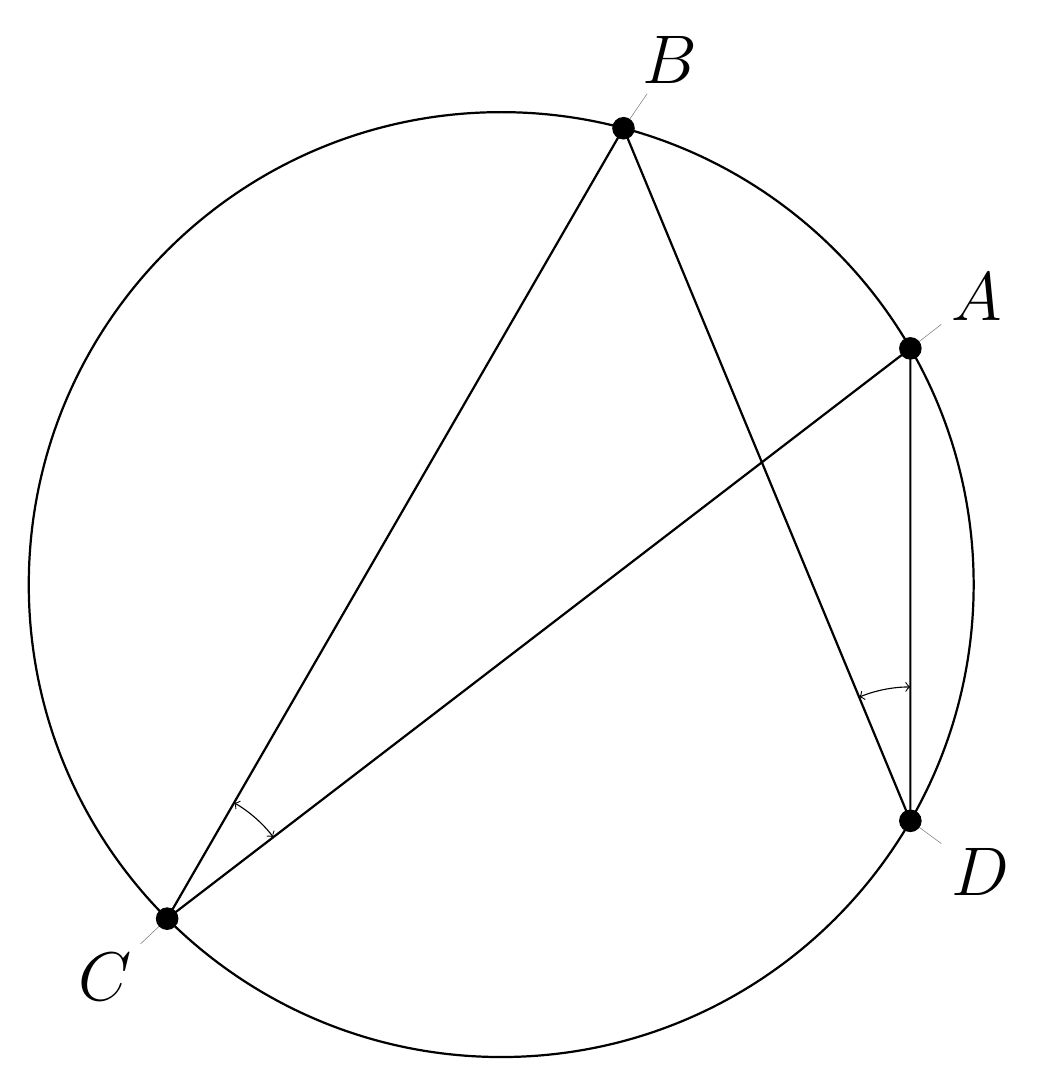
\begin{tikzpicture}[my angle/.style={draw, <->, angle eccentricity=1.3, angle radius=1.7cm}, scale = 3]
                        ]
% circle
\draw[thick] (0,0) circle (2cm);
% coordinates
\coordinate[pin= 30:{\Huge$A$}] (A) at ( 30:2);
\coordinate[pin= 75:{\Huge$B$}] (B) at ( 75:2);
\coordinate[pin= 225:{\Huge$C$}] (C) at (225:2);
\coordinate[pin= 330:{\Huge$D$}] (D) at (330:2);

\draw[fill=black] (A) circle (.3ex);
\draw[fill=black] (B) circle (.3ex);
\draw[fill=black] (C) circle (.3ex);
\draw[fill=black] (D) circle (.3ex);

% angles
\draw[thick]    (A) -- (C) -- (B);
% \pic[my angle, "\Large$\theta$"]      {angle = A--C--B};
\pic[my angle]  {angle = A--C--B};

\draw[thick]    (A) -- (D) -- (B);
\pic[my angle]      {angle = A--D--B};

\end{tikzpicture}
\end{center}

{\Huge Choose one of the following three options:}
\vspace{1cm}

{\Large $\angle ACB < \angle ADB$ \hfil $\angle ACB = \angle ADB$ \hfil $\angle ACB > \angle ADB$}
\vspace{1cm}

{\large Remember: $<$ can be read as "is less than", and $>$ can be read as "is greater than".}


\pagebreak

{\Huge \textbf{Question 2:} Given that $C$ is the centre of the circle, what is the relationship between the two marked angles, $\angle ACB$ and $\angle ADB$?}

\begin{center}
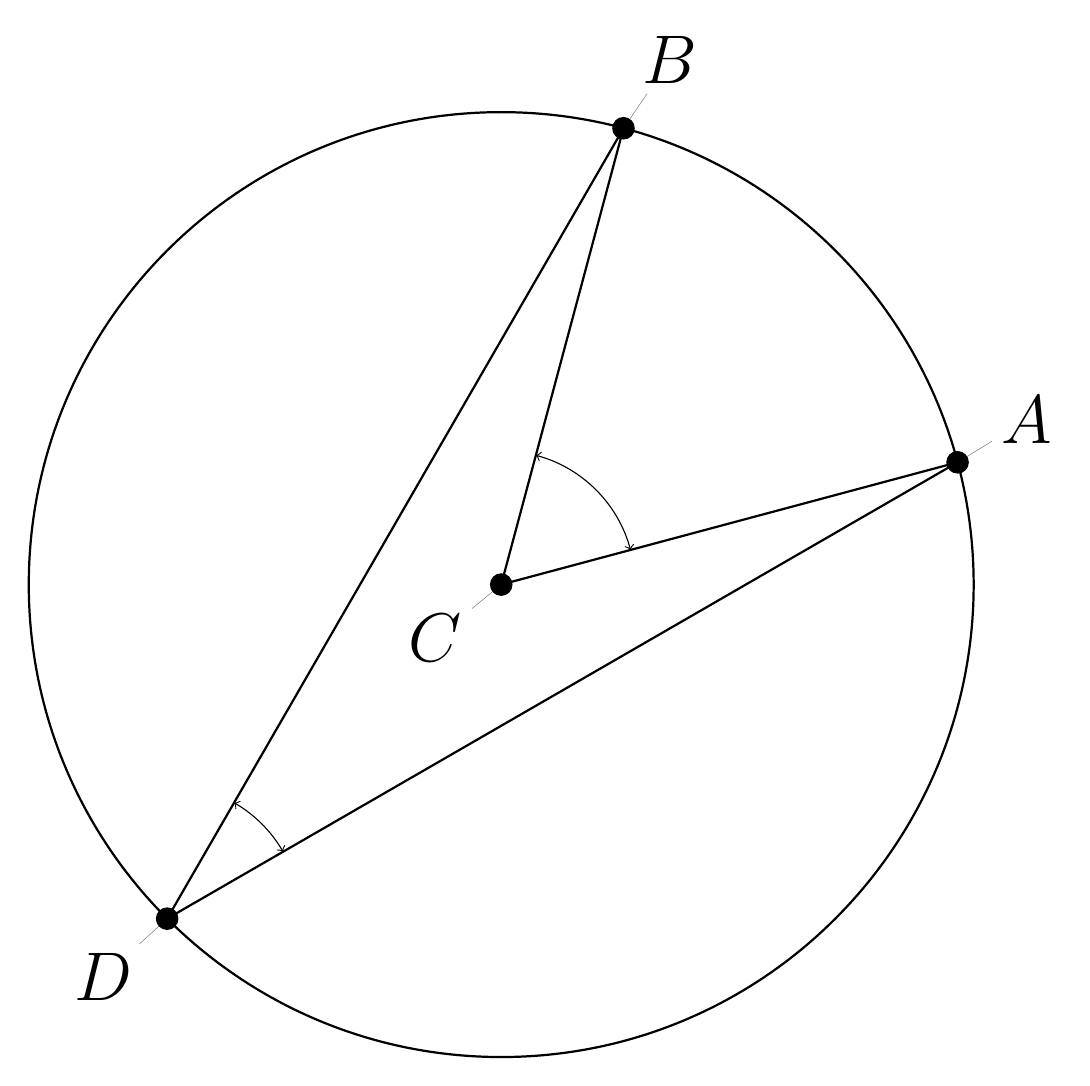
\begin{tikzpicture}[my angle/.style={draw, <->, angle eccentricity=1.3, angle radius=1.7cm}, scale = 3]
                        ]
% circle
\draw[thick] (0,0) circle (2cm);
% coordinates
\coordinate[pin= 15:{\Huge$A$}] (A) at ( 15:2);
\coordinate[pin= 75:{\Huge$B$}] (B) at ( 75:2);
\coordinate[pin= 215:{\Huge$C$}] (C) at (0, 0);
\coordinate[pin= 225:{\Huge$D$}] (D) at (225:2);

\draw[fill=black] (A) circle (.3ex);
\draw[fill=black] (B) circle (.3ex);
\draw[fill=black] (C) circle (.3ex);
\draw[fill=black] (D) circle (.3ex);

% angles
\draw[thick]    (A) -- (C) -- (B);
% \pic[my angle, "\Large$\theta$"]      {angle = A--C--B};
\pic[my angle]  {angle = A--C--B};

\draw[thick]    (A) -- (D) -- (B);
\pic[my angle]      {angle = A--D--B};

\end{tikzpicture}
\end{center}

{\Huge Choose one of the following three options:}
\vspace{1cm}

{\Large $\angle ACB = \angle ADB$ \hfil $\angle ACB = 1.5\angle ADB$ \hfil $\angle ACB = 2\angle ADB$}
\vspace{1cm}




\end{document}